\subsection{Monitoring test elink}
The test elinks (pairs of differential signals) for both data GBTxs are brought
out on the breakout board: pin 8 (P) and 10 (N); pin 34 (P) and pin 32 (N).

Please refer to
\autoref{fig:dcb-mc-reset} and \autoref{fig:dcb-tx-datavalid-pull-up} for
breakout board pinout.

Currently, we need to use the memory monitoring panel to see received packets on
MiniDAQ. Open the \textbf{MiniDAQ: TOP panel}, double click on the
\textbf{DAQ} under \textbf{Sub-System}, then double click on the \textbf{TELL40}
recursively (note that there will be suffix added to ``TELL40'') until the
following panel shows up (see \autoref{fig:mem-monitor}), then go to the
\textbf{Memory Monitoring} tab.

\begin{figure}[ht]
    \centering
    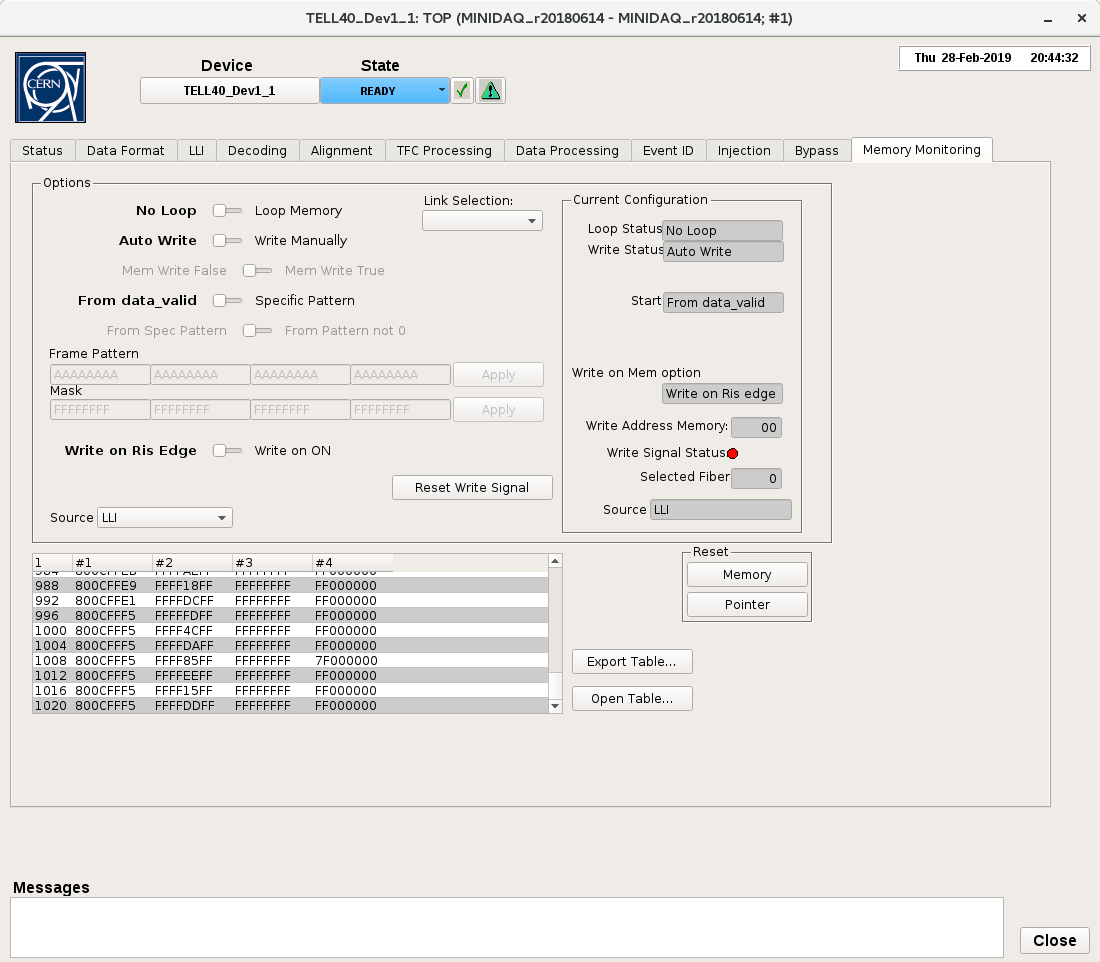
\includegraphics[width=0.9\textwidth]{res/memory_monitoring_panel.png}
    \caption{Memory monitoring panel buried in \textbf{TELL40}.}
    \label{fig:mem-monitor}
\end{figure}

Each line is a received GBT packet. The test elink data is represented by a
single Byte:

\begin{lstlisting}
800CFFF5 FFFF41FF FFFFFFFF FF000000
             ^^ test elink Byte
\end{lstlisting}
